	\chapter{Discussion}\label{cha:discussion}
	Building upon the recent findings by \citet{delaVarga2016}, the aim of this work was to extend their approach by considering practical applications and the utility structural geological modeling viewed as an Bayesian inference problem might have in an economic context. A sector in which structural geological modeling is of central importance is hydrocarbon exploration. This field is characterized by the necessity to make decisions in the face of high risks and potentially high rewards. As these decisions are often closely linked to geological modeling and the estimation of reservoir-related values, we aimed to use this context to extend the Bayesian inference step by considering its influence on respective decision-making. To observe this, a case-specific loss function was developed in this work. In doing so, we intended to furthermore show, that the loss function estimation approach is suitable and useful to describe varying degrees of complexities behind decision-making environments and the risk-related behavior of the actors in it.
	To analyze this, geological models were interpreted as potential hydrocarbon systems. A central part of our work was comprised of the development of algorithms capable of automatic structural trap recognition and subsequent calculation of values relevant to decision-making. Different prior and posterior probability distributions for such economic values were generated to form a basis for application of the custom loss function for value estimation. These methods were first applied to a conceptual 1D geological model and subsequently to a full 3D structural model. 
	Despite a significant leap in complexity, the results from both models proved to be widely similar.
	\subsubsection{State of knowledge, decision uncertainty and consequent decision making via loss function optimization}
	The economic value realized in each model construction (score and ROV, respectively), had been defined to depend on model parameters, either directly or indirectly by taking into account their relations to other parameters or to specific thresholds and conditions. This meant in general, that in this step of valuation, model uncertainties were in a way translated and reduced to the probability distribution of a single decisive value. As this was set to be the foundation for loss function estimation, we consider this value distribution to be an expression of the state of knowledge on which the decision-making is to be based. Thereby, we furthermore propose that the overall uncertainty inherent in this probability distribution can be referred to as "decision uncertainty" and that this entity is to be viewed separately from the model uncertainty.\\	
	By viewing decision-making as a problem of optimizing a case-specific loss function based on such a state of knowledge and decision uncertainty, we were able to observe clear differences in the respective behavior of distinctly risk-affine actors.
	The position and separation of their Bayes actions, i.e.\ their decisions, manifested according to the properties of the value distributions. These were in turn determined by the proportionality regarding distribution modes, their relative probabilities and distances to each other. This was often indicated by the position of mean and median relative to these modes. A mean located in the middle between two widely separated modes, which might be of low intrinsic uncertainty themselves, would indicate a much higher overall decision uncertainty, than a mean found in the middle of a narrow unimodal distribution. Pronounced bimodality between two extremes, i.e.\ high uncertainty, resulted in a wider separation of Bayes estimators. Reduction of the distribution to one mode conversely led to the convergence of different Bayes actions. A decrease in decision uncertainty furthermore was accompanied by a reduction in expected loss for each Bayes estimator. 
	Considering these observations, we derive that the degree of Bayes action convergence and respective expected losses, i.e.\ Bayes risks, can be considered measures for the state of knowledge and decision uncertainty at the moment of making a decision. The better these are, the more similar the decisions of differently risk-affine actors and the lower their loss expectations are. It can be assumed, that given perfect information, all actors would bid on the same estimate (the true value) and expect no loss, since no risk is present. It furthermore follows from this that the relevance of risk factors decreases with higher reduction of decision uncertainty.
	\subsubsection{Impact of additional information on decision making}
	Cases of various states of knowledge and decision uncertainties, i.e.\ different realizations of the value probability distribution, were attained by the implementation of Bayesian inference. While in most settings, adding information via inference led to a reduction of decision uncertainty, this was not always the case. We observed that the impact on decision uncertainty, induced by Bayesian inference, is not necessarily strictly aligned with the change in uncertainty regarding model parameters and their combinations. In respect to this, two aspects seems to be of central importance: (1) "where" in the model uncertainty is reduced, i.e.\ in which spatial area or regarding which model parameters and (2) which possible outcome is enhanced in terms of probability. An increased probability of a thick or thin seal in our 3D model, for example, equally reduced decision uncertainty significantly, by raising the probability of a positive or negative outcome, respectively. Improved certainty about our reservoir thickness, however, had little to no impact on decision-making. This shows us that some areas and parameters of the model have a much greater influence on the decision uncertainty than others.\\
	Adding to this, we observed a particular effect related to threshold values that lead to an abrupt cut-off between two extrema of decision ranges. In both types of model construction, 1D and 3D, this was directly related to sealing reliability. Thresholds regarding seal thickness (1D model) and Shale Smear Factor (SSF$_\text{c}$ in 3D model) were defined in a way that introduced a significant possibility of complete trap failure. Consequently, it was observed that reducing the uncertainty in a way that narrowed the probability of a threshold-related parameter around its cut-off value, led to an amplification of the respective mode and thus emphasized the risk of complete failure. This can be seen in the posterior ROV distribution of 3D model V (see Figure \ref{fig:ML5}). Resulting Bayes actions were characterized by an increase in divergence and expected losses, indicating a deterioration of the state of knowledge and an according increase in decision uncertainty. Thus, in some cases, adding information to the inference process might leave actors in greater disagreement than before.
	However, we furthermore have to consider that actors weight possible outcomes of the probability distribution differently. They consequently are affected differently by the same type of additional information. Risk-friendly actors were the most robust in their decision-making in the face of possible trap failure. Eliminating this risk proved to be far less significant to the most risk-friendly, than for risk-averse actors. Accordingly, it should be of foremost importance for risk-averse actors, to reduce the uncertainty regarding threshold-related factors which might decide between the success and complete failure of a project. This is less relevant for risk-friendly decisions makers, who respectively might acquire a comparable benefit from knowing more about the probability of positive outcomes, as they are less discouraged from overestimating and less afraid of failure. It was stated by \citet{bratvold2010making} that uncertainty has two possible consequences: risk and opportunity. According to them, risk is a consequence which is subjectively undesirable to an actor, while opportunity is the opposite. In our loss function, this seems to be well represented by varying affinities to rather over- or underestimate. For our risk-averse actors, a major risk is posed by seal failure. Our risk-friendliest individual sees a greater risk in missing out on opportunity. Nevertheless, it is suggested by the results from the different inference cases, that the best states of knowledge are attained by eliminating multimodality and narrowing the range of probabilities to one mode anywhere along the value axis.\\
	Crucial risks might be easily assessed, if they are dependent on only one or a few parameters, such as seal thickness in the 1D model. In other cases, they are derived from more complex parameter inter-relations, as is the case for the Shale Smear Factor, which is the ratio of displacement to seal thickness. Posterior models IV and V (see Sections \ref{sec:model4} and \ref{sec:model5}) showed that reduced uncertainty about the SSF is not necessarily directly recognizable via Shannon entropy visualization, especially if uncertainty regarding its parent parameters remains high. It follows that, to approach an effective mitigation of high risks, the complexities behind decisive factors need to be assessed thoroughly and respective parent parameters, as well as their interdependencies, need to be identified. This might enable a better understanding of which type of information is missing and where in the model additional data might be of use for improved decision-making.\\	
	%The respective estimate resilient to risk was generally found close to the positive mode and experienced only minor lateral shifting, after diminishing the probability of failure. Greater shifts were caused for this actor, in cases in which the positive mode itself was shifted laterally or erased completely. Conversely, the Bayes action of the most-averse individual was influenced greatly by the probability of the "worst case" scenario, complete trap failure. Only a stark decrease of the respective mode encouraged this actor to bid on an estimate close to the risk-friendlier decision-makers. These observations match the principles and conditions conceived in the design of the loss function and the chosen range of risk factors.	
	A central conclusion from these observations seems to be, that more of simply any type of information does not necessarily lead to better decisions. Instead, improved of decision-making is achieved by attaining the right kind of information that is able to shed light on uncertainties which are relevant to an individuals own goals and preferences, as well as the general problem at hand. These findings pair well with statements made by \citet{bratvold2010making}, who emphasized that the purpose of models in the hydrocarbon sector is to attain insights to improve decisions. In their book, they point out that value is not generated by uncertainty quantification or reduction in itself, but is created to the extent that these processes have potential to change a decision. This is reflected by our results which showed that one set of information might have a vastly different effects on a variety of Bayes estimators. New observations might lead to a great change in decision for one actor, but be negligible for the other.	
		%This state of knowledge and the decision uncertainty accordingly experienced alterations related to the different Bayesian inference cases. These changes related foremost to modes in the value distribution. For both model designs (1D and 3D), the prior value probability distributions were characterized by a distinct bimodality formed by widely separated modes of opposing values, i.e. one in the range of highly positive values, another at zero or negative values. By introducing likelihood functions, these modes were most often shifted or altered in their shape. The latter was observed as either an amplification of the mode, by raising its mean probability, while narrowing the range of probabilities (i.e.\ reducing the standard deviation), or the opposite, a diminishment of the mode up to total erasure of its probability.\\
	\subsubsection{Value distribution modes as possible model scenarios and potential decision options}	
	Effects of adding information via Bayesian inference were reflected in changing appearances of modes in the reservoir value distributions. Considering that these changes correlated with increased or decreased relevance of specific trap control mechanisms in the 3D model, we derive that each mode represents the occurrence of a specific mechanism-related scenario. These were mostly distinctly separated with little probability in between. This presumably resulted from the assumption that traps are always "filled-to-spill" in respect to spill and leak point, and that full leakage is assumed for any type of seal failure, resulting in an approximate discretization into respective scenarios.
	\begin{figure}[h]
		\centering
		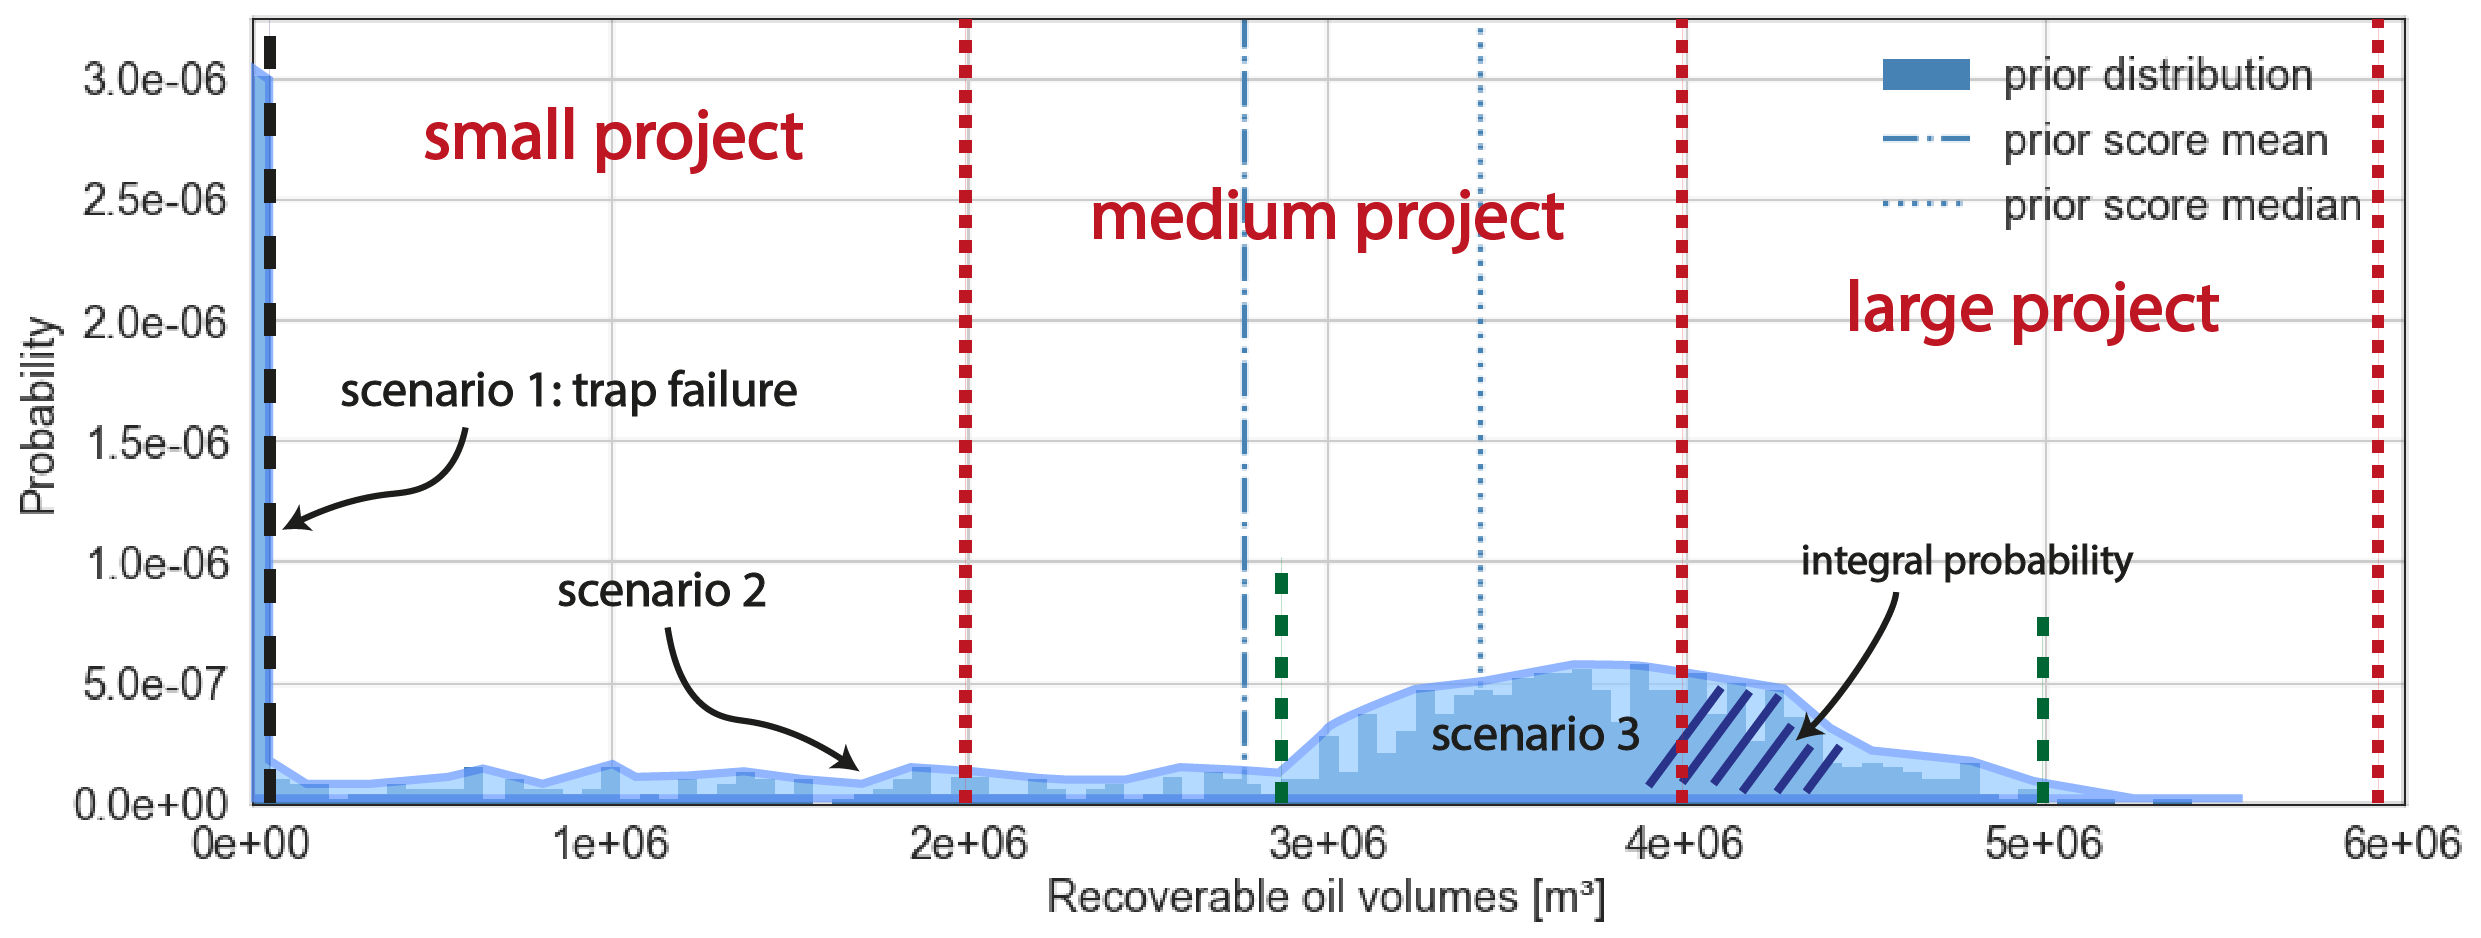
\includegraphics[width=1\textwidth]{Figures/scenarios_options}
		\caption{ROV distribution of the prior model subdivided by modes into scenarios which could pose decision options (marked by greens lines). Red lines indicate a discretization of decision options according to fixed scales of resource allocations for a project. For both cases, zero equals the option to "take no action", i.e.\ to allocate no resources.}\label{fig:scenarios_options}
	\end{figure}\\
	From a decision-making perspective, these scenarios might be interpreted as different decision options. In a case of distinct bimodality as seen in the prior of the 3D model, two main options would be given: (1) to not take any action or (2) to allocate resources according to an estimated value within the positive mode. However, most often, low probabilities for the values between these two opposite options remain. Especially considering the use of loss functions which lead to best estimates located in these areas of low probability, it is debatable, how these ranges should be treated. A possibility could be to subdivide the value probability distribution accordingly into regions. Considering respective integral probabilities for each such section and by introducing a critical integral probability as a threshold, it could be determined whether such a subregion is to be considered an actual option for decision-making or not. If a Bayes action is located outside of such a decision option, it could be automatically assigned to the closest region of sufficient integral probability. This approach should be easily applicable as an extension to our custom loss function. Furthermore, it could serve to build a bridge between this continuous loss function method and discrete approaches to structuring decision problems, such as decision trees. In real cases, normally only a limited number of options is given. In the context of hydrocarbon exploration and production, this would relate to fixed magnitudes of resource allocation, such as a certain number of required drilling wells or the size of a production platform. A discretization of decision subregions in a probability distribution could thus also be based on previously defined actual options. A schematic illustration of these concepts is shown in Figure \ref{fig:scenarios_options}, where three predefined decision areas are labeled according to hypothetical project sizes options.
	\subsubsection{Comparison to common practices and research in the hydrocarbon sector}		
	In remains to be argued, to what extent our methodology and findings contribute to practical applications in hydrocarbon exploration and production. Monte Carlo simulation for reservoir estimation and risk assessment has become common in this sector and is often used in combination with decision trees to make decisions (see \citet{murtha1997monte}, \citet{mudford2000valuing}, \citet{wim2001guidelines} and \citet{bratvold2010making}). However, it seems to us that distributions resulting from probabilistic modeling are mostly only considered to attain best estimates in the form of means. Most likely and extreme outcomes are identified as percentiles, typically P50 (the median), P10 and P90. We believe that this practice does not harness the full potential of such a probabilistic distribution and that much of the inherent information potential is discarded. Contrary to that, customized loss functions, as a Bayesian method, take into account the full probability distribution and enable the inclusion of various conditions in the process of finding an optimal estimate. While used in statistical decision theory and other scientific fields, loss functions have, to the best of our knowledge, found no significant application in the field of petroleum exploration and production. Thus, we intend to provide a new perspective with our methodology. \citet{murtha1997monte} emphasized that Monte Carlo simulation does not make decisions, it merely prepares for it. We believe that loss functions have the potential to go one step further. A hypothetical ideal loss function would consider all conditions in an economic environment, as well as perfectly represent preferences and goals of an actor and consequently be able to automatically find an optimal decision. While this is obviously unrealistic, we presume that an elaborate loss function might at least provide a very good preliminary decision recommendation. It might furthermore be able to weight risks that are not immediately apparent to an individual. Furthermore, the influence of human biases and psychological behavioral challenges, as described by \citet{bratvold2010making}, could be mitigated.\\
	More recently, Bayesian inference and MCMC methods were applied for OOIP estimation and forecasting of reservoir productivity by \citet{wadsley2005markov}, \citet{ma2006multistage} and \citet{liu2010continuous}. However, their research focused on history-matching simulations for already producing fields. Our approach of applying Bayesian inference for structural geological modeling and volumetric reservoir calculations is intended to support decision-making in the earliest stages of a reservoir, when it has to be decided whether a project should be developed or not. Nevertheless, it was shown in the research conducted by \citet{wadsley2005markov} that early volumetric OOIP estimates can be combined with later calculations from production data via MCMC methods. This is an area where our methods could possibly be integrated.\\
	\citet{bratvold2010making} highlighted the potential to use Monte Carlo simulation to identify, via sensitivity analysis, which uncertainties have the greatest impact on decisions. This was virtually achieved by performing several cases of Bayesian inference in our work, as we recognized primarily the importance of seal safety.		
	\subsubsection{Representativity and limitations of this methodology}
	It has too be emphasized that the models constructed in this work were synthetic and not based on real data. Nevertheless, the 3D model in particular was designed to include some typical structural characteristics related to hydrocarbon systems. We developed algorithms aimed to consider the most common conditions that define structural traps. The fact that similar observations were made for the 1D, as well as the 3D model, indicates a certain degree of continuity with respect to representativity. However, we also need to address that the uncertainties employed in the 3D model related to $z$-axis positional values only and were thus of primarily one-dimensional nature. This may in part account for the parallelism to the 1D model results. Furthermore, it follows that no effective uncertainty concerning the overall structural shape was implemented, particularly regarding anticlinal features and the position of the spill point in relation to the trap top. Due to this, trap volumes tended to occur primarily in distinct "filled-to-spill" scenarios. While being unrealistic, this enabled the recognition of pronounced influences related to the various control mechanisms. For computational reasons, we had to keep the number of MCMC sampling steps relatively low. For improved convergence and a higher reliability of results, more iterations should be executed. Nevertheless, we believe that for the purpose of this study, sufficient convergence and meaningful posterior results were achieved.\\	
	For a conceptual application, the customization of the loss functions was kept relatively simple. We argue that despite its simplicity, the design of the function and the incorporation of a risk factor was suitable to achieve a clear distinction between differently risk-affine actors and respective behavior. It would be possible to extend this design to attain very complex loss functions. As the loss function in this work was designed based on only a few basic assumptions, it might be more generally representative than a complex function that takes into account numerous very specific aspects. The consideration of more details, without a basis on real data, would have furthermore required extensive speculation, which would have presumably impaired the generalization potential of respective observations. We defined risk affinity to be dependent on arbitrarily chosen risk factors, which led to according re-weighting. \citet{davidson2015} used risk parameters determined by the maximal loss each actor could incur. Other approaches could be based on more tangible values, for example by making risk attitude dependent on a fixed budget. While standard loss functions only return mean or median as estimates, loss function customization offers a flexible approach to express different objective and subjective weighting factors that are specified to certain decision-making environments and decision-makers' perspectives.
	\subsubsection{Possibilities for future research and extensions}	
	Considering the findings of this work, there is still many points that could be expanded on in future research. It would be of interest to apply the same overall concept and methods on an authentic case based on real datasets. Given a realistic economic scenario, including capital and operational expenditures of a project, possibly a full net-present-value (NPV) analysis could be conducted. Recoverable reserves could be replaced by the NPV to evaluate modeling results and serve as a base for decision-making. A more elaborate respective loss function could be customized on the base of surveys, acquiring the specific preferences of one or several companies and thus attaining a better profile of the economic environment, as well as the individuals acting in it. Value of information could be considered as a parameter to better quantify the impact of Bayesian inference as observed in this work.\\
	Although the algorithms for automatic 3D hydrocarbon trap recognition were developed to fit primarily the model in this work, we presume that they could easily be adapted to other structural cases or even engineered further to be universally applicable.\\
	Furthermore, additional and different uncertainty parameters should be considered in the future. A respective next step regarding our model would be the incorporation of uncertainties which to a wider extent affect structural shapes in all three dimensions. Otherwise, non-structural reservoir parameters could be included as uncertain values, such as porosities and permeabilities of different layers. This might be of particular interest considering factors which are part of the ROV equation or other aspects that are related to high risks in decision-making.\\
	We chose hydrocarbon systems and petroleum exploration as a sector for an exemplary application in this work, but other settings can be found, in which geological modeling is of central significance for decision-making. One example would be subsurface storage of fluids in a reservoir, such as carbon capture and storage (CCS). Questions regaring storage capacity and safety deal with similar conditions and geological problems as the ones presented this work, most importantly seal reliability and the risk of leakage. In respect to this, the models and approaches in this work might provide a basis to raise new and advanced explorable cases.